\documentclass[paper=a4, fontsize=12pt]{article} % A4 paper and 11pt font size
\usepackage[T1]{fontenc} % Use 8-bit encoding that has 256 glyphs
\usepackage[english]{babel} % English language/hyphenation
\usepackage{amsmath,amsfonts,amsthm} % Math packages
\usepackage{a4wide}
\usepackage{float}
\usepackage{longtable}
\usepackage{hyperref}
\usepackage{listings}
\usepackage{makecell}
\usepackage{graphicx}
\usepackage[table]{xcolor}
\usepackage[numbered, framed]{mcode}  % To load matlab code
\lstset{deletestring=[b]{"}}

\usepackage{fancyhdr} % Custom headers and footers
\pagestyle{fancyplain} % Makes all pages in the document conform to the custom headers and footers
\setlength\parindent{0pt}
\fancyhead[L]{SF3565, Project 4, December 2016}
\fancyhead[R]{H{\"a}ggmark, Karlsson} % Empty left footer
\fancyfoot[C]{Program construction in C++ for Scientific Computing} % Empty center footer
\fancyfoot[R]{\thepage} % Page numbering for right footer

\title{Program construction in C++ for Scientific Computing \\ Teacher: Michael Hanke}

\author{Ilian H{\"a}ggmark \\ mail \href{mailto:ilianh@kth.se}{ilianh@kth.se}
  \and Andreas Karlsson \\ mail \href{mailto:andreas.a.karlsson@ki.se}{andreas.a.karlsson@ki.se} }
\date{\normalsize\today} % Today's date or a custom date

\begin{document}

\maketitle % Print the title

\section*{Project 4}
\subsection*{Task 1 - Redesign Domain class}

The Domain class is given a few new short methods to enable access to variables from the outside.\\


\subsection*{Task 2 - GFkt class}

The GFkt class holds two important objects. A Domain object that describes the grid and a matrix object that contain function values of a functon fp on the grid. Apart from the basic structure with constructor/copy-constructor etc. the GFkt class contains methods to perform basic (point-wise) aritmetic operation on the matrix containign the function values. Finaly the class have methods for calculating approximative discrete partial derivatives. \\

The first partial derivatives in $x$ and $y$ are calculated as.

$$ \frac{\partial}{\partial x} u(x_i,y_j)  = \frac{u(x_{i+1},y_j)-u(x_{i-1},y_j)}{x_{i+1} - x_{i-1}} \qquad  \frac{\partial}{\partial y} u(x_i,y_j)  = \frac{u(x_{i},y_{j+1})-u(x_{i},y_{j-1})}{y_{j+1} - y_{j-1}}$$ 

These are central derivatives that yield good accuracy, but they cannot be applied to all borders (first and last column for $x$ and firsts and last row for $y$). We therefore need one-sided derivatives to estimate the border derivatives.

$$ \frac{\partial}{\partial x} u(x_i,y_j)  = \frac{u(x_{i+1},y_j)-u(x_{i},y_j)}{x_{i+1} - x_{i}} \qquad  \frac{\partial}{\partial y} u(x_i,y_j)  = \frac{u(x_{i},y_{j+1})-u(x_{i},y_{j})}{y_{j+1} - y_{j}}$$

This would be for the first column and first row respectivley. The one-sided derivatives have lower accuracy compared to the central derivatives (see section 3). We therefore derive two a simple expression for a one-sides approximate derivative on a non equidistant grid with Talyor expansion. 


$$u(x+h_1) = u(x) + u'(x)\cdot h_1 \frac{1}{2}u''(x)\cdot h_1^2 + \mathcal{O}(h^3)$$
$$u(x+h_2) = u(x) + u'(x)\cdot h_2 \frac{1}{2}u''(x)\cdot h_2^2 + \mathcal{O}(h^3)$$

Multiply first equation with $h_2^2$ and the second with $-h_1^2$. The sum is then

$$ h_2^2 u(x+h_1)  - h_1^2 u(x+h_2)  = u(x) (h_2^2 - h_1^2 ) + u'(x) (h_1 h_2^2 - h_2 h_ 1^2) +  \mathcal{O}(h^3) $$

We neglect the higher order terms and solve for $u'(x)$

$$  u'(x) = \frac{- u(x) (h_2^2 - h_1^2 ) + h_2^2 u(x+h_1)  - h_1^2 u(x+h_2) }{h_1 h_2^2 - h_2 h_ 1^2}  $$

This approximation is marginally more complicated but gives much high accuracy. \\


For the Laplacian, $\Delta$, we can use a similar approach. The laplacian of a function $u(x,y) $ is simply $\frac{\partial^2}{\partial x^2} u(x,y) + \frac{\partial^2}{\partial y^2} u(x,y) $. The two second order derivatives can be calculated separately and then added together. Each second order derivative is calculated with a central difference. 

$$ \frac{\partial^2}{\partial x^2} u(x_i,y_j)  = \frac{u_x(x_{i+1},y_j)-u_x(x_{i-1},y_j)}{x_{i+1} - x_{i-1}} \qquad  \frac{\partial^2}{\partial y^2} u(x_i,y_j)  = \frac{u_y(x_{i},y_{j+1})-u_y(x_{i},y_{j-1})}{y_{j+1} - y_{j-1}}$$ 

where the only difference from the first order derivatives is that here the first order derivative is the input instead of the function. Also here we get the problem with border values and one-sided derivatives derived with Taylor expansion are used again.





%The discrete differential operator $\frac{\partial}{\partial x}$  can be approximated as simply $u(x+1,y)-u(x-1,y)$ and analogously for $y$. The second order %derivative can be approximated with $u(x+1,y)-2 \cdot u(x,y) + u(x-1,y)$ for the $x$-direction. The Laplacian can be expressed as 

%$$ 
% \begin{bmatrix}
%  0 & 1 &  0 \\
%  1 & -4 &  1 \\
%  0 & 1 &  0
% \end{bmatrix}
% $$
% 
% The code below shows these approximate derivatives in \textsc{Matlab}:
%
%\begin{lstlisting}
%% Approximate partial derivatives
%
%x = -30:0.1:30;
%y = -5:0.1:5;
%
%ux = sin((x/10).^2).*cos(x/10); % x-comp of u(x,y)
%[X,Y] = meshgrid(ux,y);
%u = X+Y;
%
%Dx = zeros(size(u));    % first partial derivative in x
%Dy = zeros(size(u));    % first partial derivative in y
%L = zeros(size(u));     % laplacian
%
%for i = 2:(length(x)-1)
%    for j = 2:(length(y)-1)
%        Dx(j,i) = u(j,i+1)-u(j,i-1);
%        Dy(j,i) = u(j+1,i)-u(j-1,i);
%        L(j,i) = -4*u(j,i)+u(j-1,i)+u(j+1,i)+u(j,i-1)+u(j,i+1);
%    end
%end
%\end{lstlisting}

\subsection*{Task 3 - Discrete differential operators}

The function $u(x,y)$ and its derivatives are shown below

\begin{align*}
u(x,y) &= \sin\left(\left(\frac{x}{10}\right) ^2\right ) \cos(x/10)+y \\
\frac{\partial}{\partial x} u(x,y) &= \frac{2}{100}x\cos\left(\left(\frac{x}{10}\right) ^2\right )\cos\left(\frac{x}{10}\right )- \frac{1}{10}\sin\left(\left(\frac{x}{10}\right) ^2\right )\sin\left (\frac{x}{10}\right )\\
\frac{\partial}{\partial y} u(x,y) &= \frac{\partial}{\partial y}y = 1   \\
\frac{\partial^2}{\partial x^2} u(x,y) &= \frac{2}{100}\cos\left(\left(\frac{x}{10}\right) ^2\right )\cos\left(\frac{x}{10}\right ) - \left ( \frac{2}{100}x\right )^2 \sin \left(\left(\frac{x}{10}\right) ^2\right )\cos\left(\frac{x}{10}\right ) \\
 &- \frac{2}{100}\frac{1}{10}x\cos\left(\left(\frac{x}{10}\right) ^2\right )\sin\left(\frac{x}{10}\right ) - \frac{1}{10}\frac{2}{100}x \cos\left(\left(\frac{x}{10}\right) ^2\right )\sin\left (\frac{x}{10}\right )\\
 & - \frac{1}{100}\sin\left(\left(\frac{x}{10}\right) ^2\right )\cos\left (\frac{x}{10}\right )\\
\frac{\partial^2}{\partial y^2} u(x,y) &= 0 \\
\Delta u(x,y) &= \frac{\partial^2}{\partial x^2} u(x,y) + \frac{\partial^2}{\partial y^2} u(x,y) =  \frac{\partial^2}{\partial x^2} u(x,y)
\end{align*}


The code below plot the algebraic expressions in \textsc{Matlab}. Figure \ref{fig:algebraic} shows the output.

\begin{lstlisting}
% Algebraic expressions of first and second partial derivatives in x

x = linspace(-10,5,50);		     % length set to 50 to agree with data from GFkt

figID = figure(101);                              % open figure

ux = sin((x./10).^2).*cos(x./10);                 % x-component of u(x,y)

dxu = 2/100.*x.*cos((x./10).^2).*cos(x./10) ...   % first parital derivative
      - 1/10*sin((x./10).^2).*sin(x./10);

dxxu = 2/100*cos((x./10).^2).*cos(x./10) ...      % second partial derivative
       - (2/100.*x).^2.*sin((x./10).^2).*cos(x./10) ...
       - 1/250*cos((x./10).^2).*x.*sin(x./10) ...
       - 1/100*sin((x./10).^2).*cos(x./10);
       
subplot(1,3,1); plot(x,ux);
subplot(1,3,2); plot(x,dxu);                      % plot result in subplot
subplot(1,3,3); plot(x,dxxu);

\end{lstlisting}


\begin{figure}[H]
  \centering
  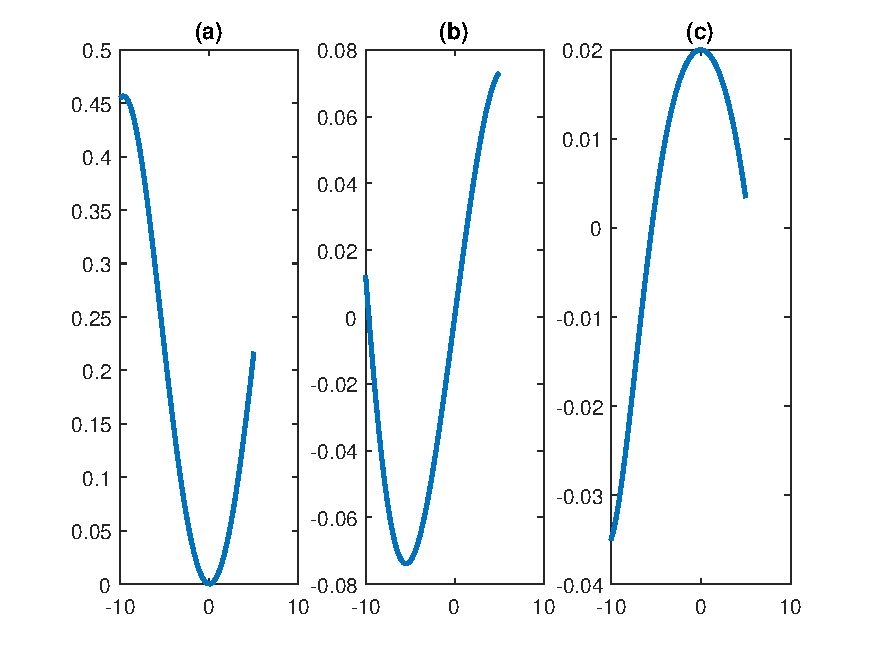
\includegraphics[width=\textwidth]{algebraicDeriv.pdf}
  \caption{\small Plot of algebraic expressions: (a) x-component of $u(x,y)$. (b) First partial derivative of $u(x,y)$ in x. (c) Second partial derivative of $u(x,y)$ in x.\label{fig:algebraic}}
\end{figure}

With the approximative derivatives implemented in task 2 we can now plot the algebraic derivatives alongside the C++ approxiamtions (Fig \ref{fig:1derivX} and \ref{fig:2derivX}). The difference between the curves is shown in blue visualize the error. We not with no surprise that the approximatice derivatives have a good arrgreement with the algebratic derivatigves in all places except the borders.


\begin{figure}[H]
  \centering
  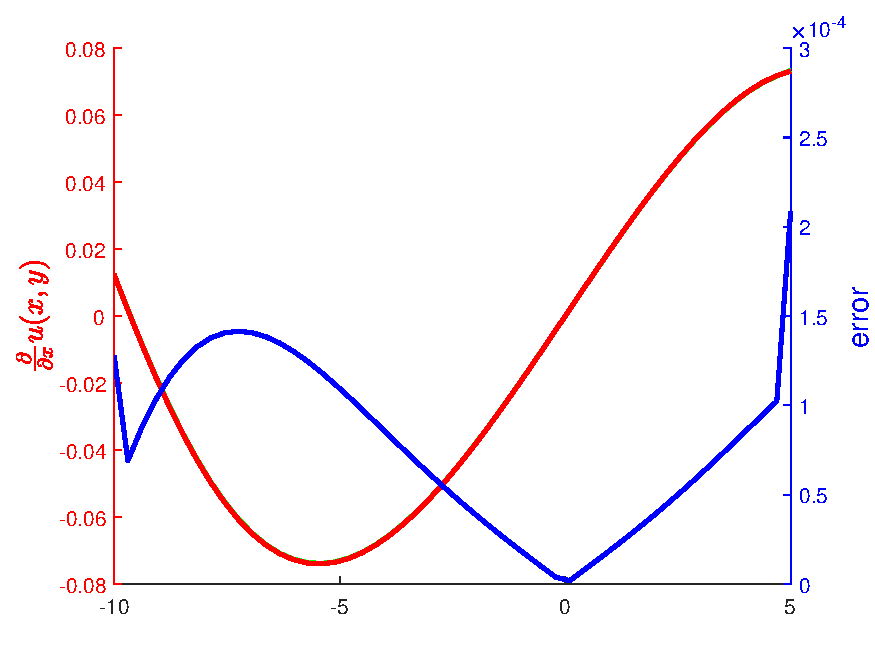
\includegraphics[width=0.8\textwidth]{comparison-x.pdf}
  \caption{\small algebraic first order x-derivative (red), approximation (green), and error (blue).\label{fig:1derivX}}
\end{figure}



\begin{figure}[H]
  \centering
  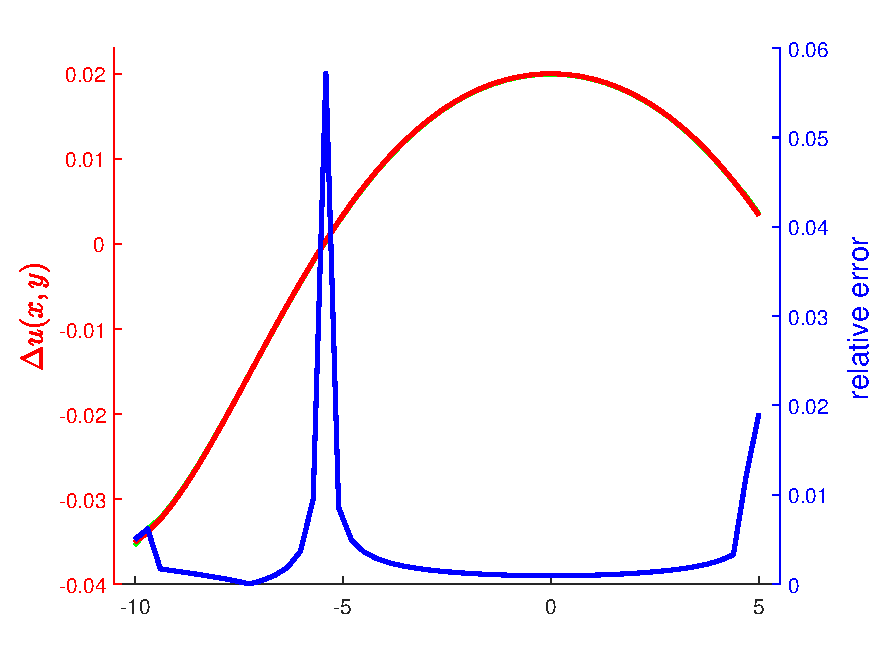
\includegraphics[width=0.8\textwidth]{comparison-xx.pdf}
  \caption{\small algebraic second order x-derivative (red), approximation (green), and error (blue).\label{fig:2derivX}}
\end{figure}


\end{document}
